\documentclass["../Cours.tex"]{subfiles}

\usepackage{mhchem}

\newcommand{\red}[1]{\textcolor{rouge}{#1}}

\begin{document}
\chapitre{Transformations du plan}

\partie{Symétrie axiale}

\begin{minipage}[t]{0.65\linewidth}
    \definition{Deux figures sont symétriques par rapport à une droite si, en <<repliant>> par rapport à la droite, les deux figures se superposent.}
\end{minipage}\hspace{0.05\linewidth}
\begin{minipage}[t]{0.3\linewidth}
    \illustration{
        \begin{centre}
            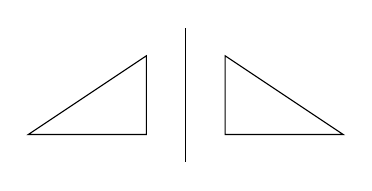
\begin{tikzpicture}[scale=0.5]
                \draw (1,0) -- +(3,0) -- +(0,2) -- cycle;
                \draw[xscale=-1] (1,0) -- +(3,0) -- +(0,2) -- cycle;
                \draw (0,2.7) -- (0,-0.7);
            \end{tikzpicture}
        \end{centre}    
    }
\end{minipage}

\newcommand{\bleu}[1]{\textcolor{bleu}{#1}}%
\propriete{La symétrie axiale est une isométrie :
\begin{itemize}
    \item conservation de la nature : \bleu{(le symétrique d'un cercle est un cercle)}
    \item conservation des longueurs : \bleu{(le symétrique d'un segment de longueur \qty{2}{\centi\metre} fait \qty{2}{\centi\metre})}
    \item conservation des angles : \bleu{(le symétrique d'un angle de \ang{30} fait \ang{30})}
\end{itemize}
}

\exemple{Tracer le triangle $ABC$ tel que $AB=\qty{6}{\centi\metre}$, $AC=\qty{5}{\centi\metre}$ et $BC=\qty{4}{\centi\metre}$,\\ puis tracer le symétrique du point $C$ par rapport à la droite $(AB)$.
\begin{centre}
    \color{noir}%
    \begin{tikzpicture}[scale=1]
        \draw[dashed] (-3,0) -- (9,0);
        \draw (0,0) node[below]{$A$} -- (6,0) node[below]{$B$} -- (3.75,3.31) node[right]{$C$} -- cycle;
        \draw[rouge] (3.75,3.31) -- (3.75,0) node[midway]{\_} -- (3.75,-3.31) node[midway]{\_} node[right]{$C'$};
        \fill[rouge] (3.75,0) rectangle +(0.2,0.2);
    \end{tikzpicture}
\end{centre}
}

\propriete{$C'$ est le symétrique de $C$ par rapport à $(AB) \Longleftrightarrow (AB)$ est la médiatrice de $[CC']$.}

\partie{Symétrie centrale}

\definition{Deux figures sont symétriques par rapport à un point (centre de symétrie) lorsqu'en faisant tourner la première figure autour du centre, on obtient la deuxième figure au bout d'un demi-tour.}

\illustration{
    \begin{centre}
        \begin{tikzpicture}
            \draw (1,0.5) -- +(3,0) -- +(0,2) -- cycle;
            \draw[xscale=-1,yscale=-1] (1,0.5) -- +(3,0) -- +(0,2) -- cycle;
            \draw[dashed] (1,0.5) -- (-1,-0.5);
            \fill (0,0) circle (0.075) node[below right]{$O$};
            \draw[-Latex,rouge] (2,1) arc(26.57:-150:{sqrt(5)}) node[midway,below right]{\scriptsize{demi-tour}};
            \fill[vert!70!white] (2,1) circle (0.09);
            \fill[vert!70!white] (-2,-1) circle (0.09);
        \end{tikzpicture}
    \end{centre}
}

\propriete{$A'$ est le symétrique du point $A$ par rapport à $O \Longleftrightarrow OA=OA'$ et O, A, $A'$ sont alignés.}

\propriete{La symétrie centrale est une isométrie.}

\clearpage
\partie{Translation}

\definition{Une translation est un déplacement rectiligne dans le plan.}

\propriete{Une translation est une isométrie.}

\illustration{
    \begin{centre}
        \begin{tikzpicture}
            \draw (0,2) node[above]{$A$} -- ++(0,-2) node[below]{$B$} -- ++(3,0) node[below]{$C$} -- cycle;
            \draw (6,2) node[above]{$A'$} -- ++(0,-2) node[below]{$B'$} -- ++(3,0) node[below]{$C'$} -- cycle;
            \draw[-Latex, rouge] (0,2) -- (6,2) node[midway,above]{\qty{6}{\centi\metre}};
        \end{tikzpicture}
    \end{centre}
}

\notation{
    \begin{itemize}
        \item La translation qui transforme $A$ en $A'$.
        \item La translation de \emph{vecteur} $\overrightarrow{AA'}$.
        \item $C'$ est l'image de $C$ par cette translation.
    \end{itemize}
}

\clearpage
\EXERCICES
\begin{questions}
    \exercice $ABCD$ est un parallélogramme.\\
    $O$ est l'intersection des diagonales de $ABCD$.
        \question Tracer la figure avec $AB=\qty{5}{\centi\metre}$, $BC=\qty{3}{\centi\metre}$ et $\widehat{ABC}=\ang{60}$.
        \question Démontrer que $A$ est le symétrique de $C$ par rapport à $O$.
        \question Sans justifier, donner le symétrique de $ABC$ par rapport à $O$.
    \exercice $[AB]$ est un segment de longueur \qty{1}{\centi\metre}.
    \begin{itemize}
        \item $A_1$ est le symétrique de $A$ par rapport à $B$.
        \item $A_2$ est le symétrique de $A$ par rapport à $A_1$.
        \item $A_3$ est le symétrique de $A$ par rapport à $A_2$.
        \item $A_4$ est le symétrique de $A$ par rapport à $A_3$.
    \end{itemize}
        \question Quelle est la longueur de $[AA_4]$ ?
        \question On réitère la construction avec $A_5$, $A_6$, $A_7$, etc. Trouver le plus petit $n$ tel que $AA_n > \qty{100}{\metre}$.

    \exercice On considère le pavage ci-dessous, constitué de droites parallèles.

    \begin{minipage}[m]{0.2\linewidth}
        \begin{center}
            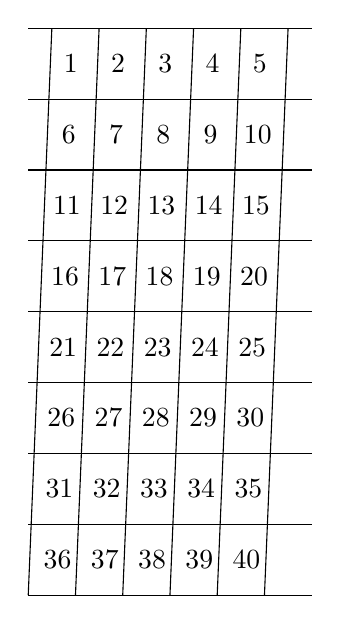
\begin{tikzpicture}[xscale=0.6,yscale=0.9]
                \foreach \y in {0,...,8} {
                    \draw (0,-\y) -- ++(6,0);
                }
                \foreach \x in {0,...,5} {
                    \draw (\x+0.5,0) -- ++(-0.5,-8);
                }
                \foreach \i in {1,...,40} {
                    \node at ({0.9+mod((\i-1),5)-0.04*int((\i-1)/5)},{-int((\i-1)/5)-0.5}) {\i};
                }
            \end{tikzpicture}
        \end{center}
    \end{minipage}
    \begin{minipage}{0.8\linewidth}
        \question 
            \subquestion Quelle est la nature du quadrilatère $ABCD$ ?
            \subquestion Quelle est l'image du point $D$ par la translation qui transforme $C$ en $B$ ?
            \subquestion Quelle est l'image du point $C$ par la translation qui transforme $B$ en $A$ ?
        \question Soit la translation qui transforme $F$ en $G$.
            \subquestion Quelle est l'image du motif 13 ?
            \subquestion Quelle est l'image du motif 16 ?
            \subquestion Quelle est l'image du motif 32 ?
        \question Soit la translation qui transforme $E$ en $H$.
            \subquestion Quelle est l'image du motif 13 ?
            \subquestion Quelle est l'image du motif 16 ?
            \subquestion Quelle est l'image du motif 32 ?
        \question Soit la translation qui transforme $B$ en $C$.
            \subquestion Quelle est l'image du motif 9 ?
            \subquestion Quelle est l'image du motif 12 ?
            \subquestion Quelle est l'image du motif 16 ?
            \subquestion Quelle est l'image du motif 23 ?
        \question Soit la translation qui transforme $E$ en $G$.
            \subquestion Quelle est l'image du motif 9 ?
            \subquestion Quelle est l'image du motif 12 ?
            \subquestion Quelle est l'image du motif 16 ?
            \subquestion Quelle est l'image du motif 23 ?
        \question 
            \subquestion Le motif 15 est l'image du motif 32 par une translation. Laquelle ?
            \subquestion En utilisant la même translation, quelle est l'image du motif 26 ?
            \subquestion Et du motif 37 ?
    \end{minipage}    
\end{questions}

\begin{comment}
\clearpage
\begin{questions}

\newcommand{\cor}[1]{{\color{rouge}#1}}

\textbf{Étape 1}

\question L’alginate de sodium est une espèce chimique comestible et soluble dans l’eau. Elle a pour formule chimique \ce{C_6 H_7 O_6 Na}.
\subquestion Préciser le nombre d’atomes d’oxygène dans cette formule chimique.

\cor{Il y 6 atomes d'Oxygène dans cette molécule, on le sait grâce au petit 6 en bas à droite du symbole \ce{O} dans la formule chimique. << \ce{O_6} >>}

\subquestion Le numéro atomique de l’atome d’oxygène est $Z = 8$, cela signifie qu’il comporte 8 protons. Indiquer le nombre d’électrons présents dans un atome d’oxygène.

\cor{Un atome a autant de protons que d'électrons. Donc si l'atome d'Oxygène a 8 protons, il a aussi 8 électrons.}

\question Pour préparer la solution d’alginate de sodium, on verse \qty{8}{\gram} d’alginate de sodium solide dans \qty{100}{\gram} d’eau et on mélange jusqu’à la dissolution complète. On mesure la masse $m$ de la solution obtenue, on obtient $m = \qty{108}{\gram}$. Interpréter ce résultat expérimental en raisonnant sur l’évolution de la masse au cours de la dissolution.

\cor{Au cours de la dissolution, la masse des éléments est conservée. C'est pourquoi la masse finale \qty{108}{\gram} est égale à la somme des masses de départ $\qty{8}{\gram} + \qty{100}{\gram}$.}

\vspace{2ex}
\textbf{Étape 2}

\question Pour obtenir des billes de grande taille, on place la solution d’alginate de sodium au congélateur. Après plusieurs heures, elle devient solide. Indiquer, en le justifiant, si la solution d’alginate de sodium subit une transformation chimique ou une transformation physique.

\cor{En plaçant l'alginate de sodium au congélateur, sa température a diminué jusqu'à \emph{changer d'état} et passer de l'état liquide à l'état solide. C'est donc une transformation physique que l'on appelle << solidification >>.}

\vspace{2ex}
\textbf{Étape 3}

L’étape finale de la production de ces billes consiste à faire réagir des ions alginate de formule \ce{C6H7O6^-} avec l’élément calcium sous la forme \ce{Ca^2+} pour former une paroi gélifiée d’alginate de calcium de formule chimique \ce{C12H14O12Ca}. L’équation de la réaction permettant de modéliser cette étape s’écrit : 

\centerline{\ce{2 C6H7O6^- + Ca^2+ -> C12H14O12Ca}}

\question Donner la formule chimique de chacun des réactifs.

\cor{Les réactifs sont ceux situés à gauche de la flèche, donc \ce{C6H7O6^-} et \ce{Ca^2+}.}

\question Lors de la transformation chimique, \red{deux ions} alginate réagissent avec un \red{ion de calcium} pour former \red{de l'alginate de calcium}.

\begin{itemize}
    \item << deux ions alginate >> car dans l'équation on a << \ce{\red{2} C6H7O6^-} >>
    \item << ion de calcium >> et pas "atome de calcium", car dans l'équation \ce{Ca} est le symbole du calcium et on a << \ce{Ca^2+} >> (s'il y a un + ou un - en haut à droite du symbole, c'est un ion, sinon c'est un atome)
    \item << de l'aginate de calcium >>, c'est le non du produit qui a pour formule \ce{C12H14O12Ca} (donné dans la question)
\end{itemize}

\clearpage
\textbf{Étape 4}
\question Dans cette partie, on s’intéresse au poids de la solution d’alginate de sodium contenue dans la bille figurant sur la photo. Déterminer la valeur du poids de la solution d’alginate de sodium contenue dans la bille
figurant sur la photo, à l’aide des données suivantes :
\begin{itemize}
    \item Les photos sont à l’échelle $1/2$ : \qty{1}{\centi\metre} sur la photo représente \qty{2}{\centi\metre} en réalité.   
    \item La masse volumique de la solution d’alginate de sodium a pour valeur \qty{1.1}{\gram\per\centi\metre\cubed}.
    \item Pour calculer le volume $V$ d’une bille de rayon $R$, de diamètre $D$, il est possible d’utiliser l’une des relations suivantes :
    \begin{itemize}
        \item $V=\num{0.52} \times D^3$
        \item $V=\num{4.2} \times R^3$
        \item $V=\frac{4}{3} \pi R^3 $
    \end{itemize}
    \item L’intensité de la pesanteur a pour valeur $g = \qty{9.8}{\newton\per\kilo\gram}$.
    \item Si besoin, le segment gradué ci-joint est utilisable.
\end{itemize}

{\color{rouge}
    
    On demande de calculer le \emph{poids} de la solution d'alginate de sodium. Pour calculer le poids, on utilise la formule $P= m \times g$. Mais on ne connaît pas $m$ la masse.\\

    Pour la calculer la masse, on peut utiliser la masse volumique $\rho$ donnée dans l'énoncé : $m = \rho \times V$. Mais on ne connaît pas $V$ le volume.\\

    Pour calculer le volume, on peut utiliser une des formules données dans l'énoncé, par exemple celle-ci : $V=\num{0.52} \times D^3$. Mais on ne connaît pas $D$ le diamètre.\\

    Toutefois, grâce au schéma donné dans l'énoncé, on peut mesurer le diamètre.\\

\fbox{
    \begin{minipage}{\linewidth}
        \textbf{Étapes de raisonnement}
        \begin{enumerate}
            \item Mesurer le diamètre.
            \item Calculer le volume en utilisant le diamètre
            \item Calculer la masse en utilisant la masse volumique et le volume
            \item Calculer le poids en utilisant la masse et l'intensité de la pesanteur $g$.
        \end{enumerate}
    \end{minipage}
}

    \begin{enumerate}
        \item Sur le schéma, je mesure que $D=\qty{1.9}{\centi\metre}$. Comme on est à l'échelle $1/2$, la vraie valeur est 2 fois plus grande, donc le vrai diamètre vaut $D=\qty{3.8}{\centi\metre}$.

        \item Je calcule le volume :
        \begin{align*}
            V &= \num{0.52} \times D^3 \\ 
            V &= \num{0.52} \times \num{3.8}^3 \\ 
            V &\approx \qty{28.5}{\centi\metre\cubed}
        \end{align*}

        \item Je calcule la masse : 
        \begin{align*}
            m &= \rho \times V \\ 
            m &= \num{1.1} \times \num{28.5} \\
            m &= \qty{31.4}{\gram}
        \end{align*}

        \item Je calcule le poids : 
        \begin{align*}
            P &= m \times g \\ 
            P &= \qty{31.4}{\gram} \times \num{9.8} \\ 
            P &= \qty{31.4e-3}{\kilo\gram} \times \num{9.8} \\ 
            \Aboxed{P &= \qty{0.307}{\newton}}
        \end{align*}

    \end{enumerate}
}

\end{questions}
\end{comment}

\end{document}